\subsection*{Pandas Dataframe operations}
A dataframe can be thought of as a 2D list (list within a list) supporting access in more semantic, meaningful ways compared to using indices. Visualized, a dataframe may look something like the following: 

{\centering
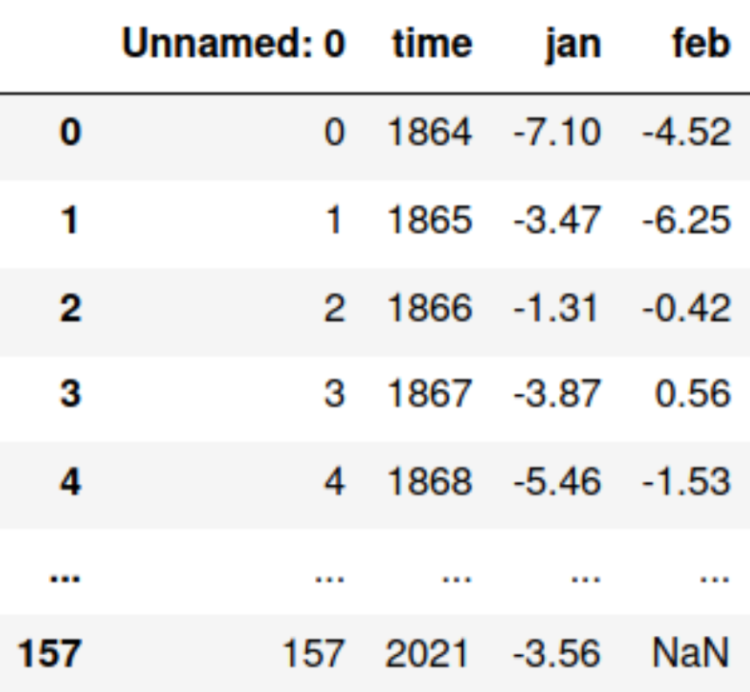
\includegraphics[width=0.8\linewidth]{src/10_pandas/images/pd_dataframe_index.png}\\
table of the climate, entries accessible via index \par}

The leftmost column is known as the "index column".  

{\centering\underline{\textbf{Change the Index Column}} \par}
\begin{lstlisting}
climate2 = climate.set_index("time") #creates copy
\end{lstlisting}
{\centering
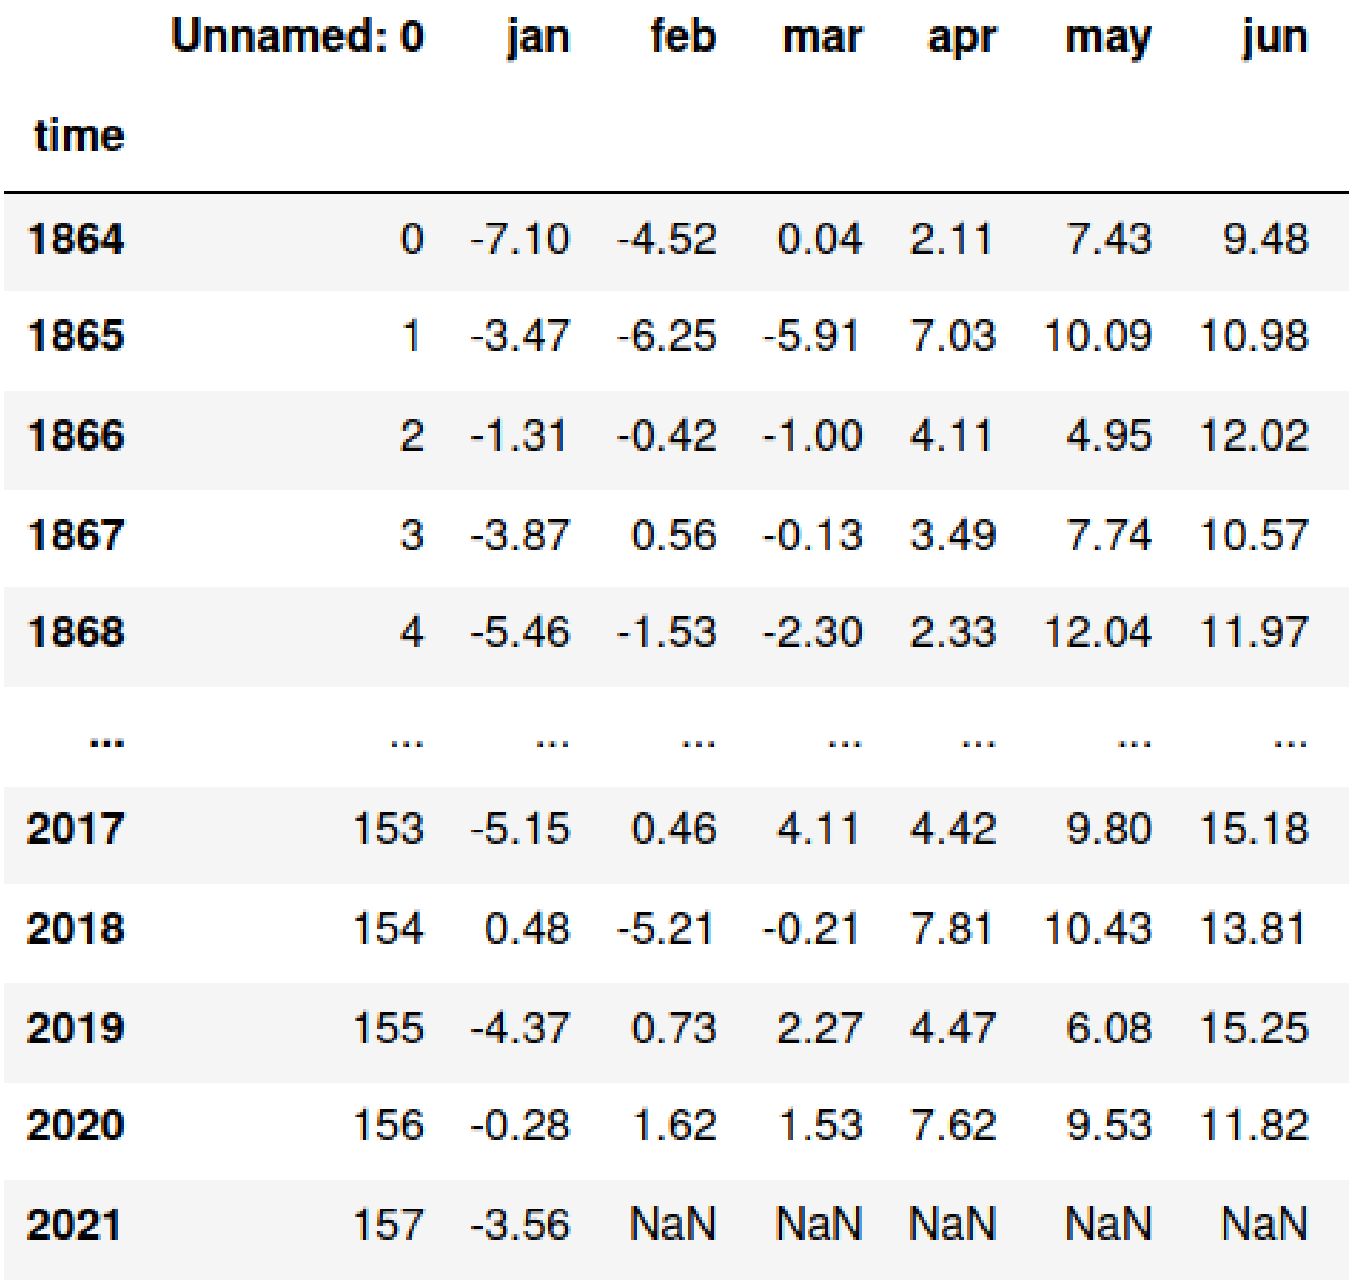
\includegraphics[width = 0.8\linewidth]{src/10_pandas/images/pd_dataframe_time.png}\\
table of the climate, entries accessible via time \par}

{\centering\underline{\textbf{Rename Columns}} \par}
\begin{lstlisting}
climate = climate.rename(columns={"old_index_name":"new_index_name", ...})
#renames the "old_index_name" column to "new_index_name"
\end{lstlisting}
rename all columns (len(data.columns) = number of colums must be true)
\begin{lstlisting}
data.columns = ["Date", "January", "February", ...]
\end{lstlisting}

{\centering\underline{\textbf{Access Dataframe Elements}} \par}
Access a single column (type: Series):
\begin{lstlisting}
climate["feb"]
#gets the column "feb"
\end{lstlisting}
Access multiple columns (type: Dataframe):
\begin{lstlisting}
climate[["jan", "mar"]]
#gets the columns "jan" and "mar"
\end{lstlisting}
Access a single row, using an index (type: Series):
\begin{lstlisting}
climate.iloc[3]
#gets row 3
\end{lstlisting}
Multiple rows (type: Dataframe):
\begin{lstlisting}
Climate.iloc[1:4]
#gets rows 1 to 3
\end{lstlisting}
Access to a subtable using indices (type: Dataframe):
\begin{lstlisting}
climate.iloc[4:7,1:2]
#gets rows 4,7 with data only from column 1
\end{lstlisting}
Access to a subtable using index column values and column name (type: Dataframe):
\begin{lstlisting}
climate2 = climate.set_index("time")
climate2.loc[1864:1868,"jan":"mar"]
#includes the rows labeled with 1864 until and including #1868, the columns from "jan" until and including "mar"
\end{lstlisting}
Access to a single element:
\begin{lstlisting}
climate["jan"][3]
#gets the element in column "jan" in row 3
\end{lstlisting}

{\centering\underline{\textbf{Filter Dataframes}} \par}
Filter rows:
\begin{lstlisting}
climate[climate["jan"]>2]
#filters out the rows with values in the "jan" column #less than 2
\end{lstlisting}
• Example: All entries in "jan" with values more than 2:
\begin{lstlisting}
climate["jan"][climate["jan"]>2]
\end{lstlisting}

{\centering\underline{\textbf{Dealing with Invalid Data}} \par}
Convert all the values in a column to numeric:
\begin{lstlisting}
data[column] = pd.to_numeric(data[column], errors="coerce")
#converts all the values to numeric values. #errors="coerce" -> converts values which cannot be #converted to NaN.
\end{lstlisting}
Delete all rows containing NaN entries:
\begin{lstlisting}
data.dropna(axis = 0, how="any")
#how="any" -> delete row if any value is NaN.
#how="all" -> delete row if all values are NaN
#axis = 1 -> delete column instead of row
\end{lstlisting}
• Fill all entries containing NaN with a value:
\begin{lstlisting}
data.fillna(0) #fill any NaN entries with 0
\end{lstlisting}

{\centering\underline{\textbf{Modify Dataframes}} \par}
Add a column:
\begin{lstlisting}
climate["new_col"] = climate["time"] + climate["jan"] 
#"new_col" is a new column whose values are #those of the "time" and "jan" column added
\end{lstlisting}
Delete a column:
\begin{lstlisting}
climate = climate.drop(columns=["time"])
#delete the "time" column
\end{lstlisting}
Add a row:
\begin{lstlisting}
d = {"mar":34, "jan":23}
climate.append(d, ignore_index=True)
#adds another row with the values 34 for "mar" and 23 for #"jan". Other entries are NaN
\end{lstlisting}
Delete a row:
\begin{lstlisting}
climate = climate.drop(climate.index[0]) 
#deletes row 0
\end{lstlisting}
Transpose the dataframe:
\begin{lstlisting}
climate = climate.T
\end{lstlisting}

{\centering\underline{\textbf{Analyse Data}} \par}
Sum of all the entries in each column (type: Series):
\begin{lstlisting}
climate.sum()
\end{lstlisting}
Maximum of all the entries in each column (type: Series):
\begin{lstlisting}
climate.max()
\end{lstlisting}
Create a dataframe summarizing the max and sum for each column:
\begin{lstlisting}
climate.agg(["max","sum"])
#A dataframe containing the same columns as climate
#with row 0 containing the max of the column and row 1 #containing the sum of the column. The strings in the 
#list should be names of valid pandas Series functions. 
\end{lstlisting}
Get statistical information for each column (type: Dataframe):
\begin{lstlisting}
climate.describe()
#includes a variety of statistical measures
\end{lstlisting}
Sort a dataframe according to entries in a specific column(s):
\begin{lstlisting}
climate = climate.sort_values(["time", "jan"], ascending=False)
#sorts the rows by "time" in descending order. If two #entries for "time" are equal, then the rows are sorted #by "jan"
\end{lstlisting}
Split a dataframe into groups based on a specified column and perform a computation on each group:
\begin{lstlisting}
data.groupby("column").sum() 
#groups data based on the entries for "column" and #calculates the sum for each group.
data.groupby("column").max()
#groups data based on the entries for "column" and #calculates the max for each group.
\end{lstlisting}